\documentclass{emulateapj}
%\documentclass[12pt,preprint]{aastex}

\usepackage{graphicx}
\usepackage{float}
\usepackage{amsmath}
\usepackage{epsfig,floatflt}
\usepackage{hyperref}
\usepackage[toc, page]{appendix}
\usepackage{verbatim, amsmath, amsfonts, amssymb, amsthm}
\usepackage[utf8]{inputenc}
\usepackage{textcomp}
\usepackage{float}
\usepackage{xcolor}
\usepackage{color}
\usepackage{listings}
\usepackage{fancyhdr}
\usepackage[T1]{fontenc}
\usepackage{url}
\usepackage[export]{adjustbox}
\usepackage{calc}

\usepackage{accents}
\newcommand{\dbtilde}[1]{\accentset{\approx}{#1}}
\newcommand{\vardbtilde}[1]{\tilde{\raisebox{0pt}[0.85\height]{$\tilde{#1}$}}}

\usepackage{lipsum}
\usepackage[para]{footmisc}


\definecolor{mygreen}{rgb}{0,0.6,0}
\definecolor{mygray}{rgb}{0.5,0.5,0.5}
\definecolor{mymauve}{rgb}{0.58,0,0.82}

\lstset{ %
	backgroundcolor=\color{white}\ttfamily\tiny,   % choose the background color; you must add \usepackage{color} or \usepackage{xcolor}; should come as last argument
	basicstyle=\tiny,        % the size of the fonts that are used for the code \footnotesize,
	breakatwhitespace=false,         % sets if automatic breaks should only happen at whitespace
	columns=fullflexible,    %no spaces between columns
	keepspaces=true,
	breaklines=true,                 % sets automatic line breaking
	breakatwhitespace=true,
	captionpos=b,                    % sets the caption-position to bottom
	commentstyle=\color{mygreen},    % comment style
	deletekeywords={...},            % if you want to delete keywords from the given language
	escapeinside={\%*}{*)},          % if you want to add LaTeX within your code
	extendedchars=true,              % lets you use non-ASCII characters; for 8-bits encodings only, does not work with UTF-8
	frame=single,	                   % adds a frame around the code
	keepspaces=true,                 % keeps spaces in text, useful for keeping indentation of code (possibly needs columns=flexible)
	keywordstyle=\color{blue},       % keyword style
	language=Python,                 % the language of the code
	morekeywords={*,...},           % if you want to add more keywords to the set
	%numbers=left,                    % where to put the line-numbers; possible values are (none, left, right)
	%numbersep=5pt,                   % how far the line-numbers are from the code
	%numberstyle=\tiny\color{mygray}, % the style that is used for the line-numbers
	rulecolor=\color{black},         % if not set, the frame-color may be changed on line-breaks within not-black text (e.g. comments (green here))
	showspaces=false,                % show spaces everywhere adding particular underscores; it overrides 'showstringspaces'
	showstringspaces=false,          % underline spaces within strings only
	showtabs=false,                  % show tabs within strings adding particular underscores
	stepnumber=1,                    % the step between two line-numbers. If it's 1, each line will be numbered
	stringstyle=\color{mymauve},     % string literal style
	tabsize=1,	                   % sets default tabsize to 2 spaces
	%title=\lstname                   % show the filename of files included with \lstinputlisting; also try caption instead of title
}

\begin{document}

\title{Comparing efficiency of different algorithms for solving sets of linear equations}

\author{Bruce Chappell and Markus Bjørklund}

\email{markus.bjorklund@astro.uio.no}

\altaffiltext{1}{Institute of Theoretical Astrophysics, University of
  Oslo, P.O.\ Box 1029 Blindern, N-0315 Oslo, Norway}

\begin{abstract}
In this letter we analyze and compare the efficiency of a general, tailored and a LU-decomposition algorithm to solve a set of linear equations. The problem we will focus on is a discretized approximation to the one dimensional Poisson equation. The results show that, for n equations, we get $8n-7$ floating point operations (FLOPS) for the general algorithm, $4n-3$ FLOPS for the tailored algorithm and $\frac{2}{3}n^3$ FLOPS for the LU-decomposition method. We found that the optimal step length is $h=10^{-7}$. The results also show that the LU decomposition can not handle cases where the matrix is bigger or equal to $n=10^5$, whilst the other algorithms handle this very well.

\end{abstract}
\keywords{Algorithm efficiency --- Linear algebra: simulation --- methods: computational}

\section{Introduction}
\label{sec:introduction}
Solving differential equations is an integral part of most research today. For most differential equations there exists no analytic solution, so we have to use a computational approach. Generally, the more realistic the model is, the more complex it is, and therefore more computationally demanding. There would be a lot to gain to increase efficiency on the algorithms used to solve such equations, thereby allowing for more efficient memory usage to solve more complex problems or increase the resolution of a given discretization. We have presented theory for the different algorithms in the method section, provided results for CPU runtime and error estimation in the results section, and drawn some conclusions. We have also proposed future steps in the further research section.

In this letter we will adopt a numerical approach to solving the one dimensional Poisson equation, which shows up in numerous areas of science.

\section{Method}
\label{sec:method}
This section will describe the methods we utilized to acquire our results.
\subsection{Model}
We want to solve the one dimensional Poisson equation shown in equation \ref{eq:poisson}.

\begin{equation} \label{eq:poisson}
    -\frac{d^2u(x)}{dx^2} = f(x).
\end{equation}
We confine the equation to a normalized interval and with Dirichlet boundary conditions, namely

\begin{equation} \label{eq:conditions}
    x \in [0,1]\text{   } , \text{   } u(0) = u(1) = 0.
\end{equation}
For reference, we assume the source term to be
\begin{equation} \label{eq:fofx}
    f(x) = 100e^{-10x}.
\end{equation}
The equation then has an analytic solution in
\begin{equation} \label{eq:analytic}
    u(x) =1 - \left(1-e^{-10}\right)x - e^{-10x}. 
\end{equation}

We discretize the interval to $n+2$ points, so that $x_0 = 0$ and $x_{n+1} = 1$, giving a step length of $h = \frac{1}{n+1}$. We approximate the second derivative to the second order, giving equation \ref{eq:approx} for a point $f(x_i)$:

\begin{equation} \label{eq:approx}
    - \frac{v_{i+1} + v_{i-1} - 2v_{i}}{h^2} = f_i
\end{equation}
This can be rewritten as 

\begin{equation}
    -v_{i-1} + 2v_{i} - v_{i+1} = f_i \cdot h^2
\end{equation}
for $i=1,...,n$ and the end points decided by the boundary conditions. We then get a set of n equations like following

\begin{align*}
    - v_{0} + 2v_{1} - &v_{2} = f_1 \cdot h^2 \\
    - v_{1} + 2&v_{2} - v_{3} = f_2 \cdot h^2 \\
    - &v_{2} + 2v_{3} - v_{4} = f_3 \cdot h^2 \\
    \vdots
\end{align*}
Written as a matrix equation, this produces the equation

\begin{equation}
    \bold{A}\bold{v} = \bold{\tilde{f}}
\end{equation}
with $\bold{\tilde{f}} = \bold{f}\cdot h^2$ and the tri-diagonal $n \times n$ matrix

\begin{equation} \label{eq:specialmatrix}
    \bold{A} = \left( \begin{array}{cccc}
2 & -1 & & 0\\
-1 & \ddots & \ddots & \\
& \ddots & \ddots & -1 \\
0 & & -1 & 2 \end{array} \right) .
\end{equation}

\subsubsection{General case}
We first address the general case, where we don't assume the values of the upper, lower and main diagonal. Adopting separate names for the three diagonals, $\bold{a}$,$\bold{b}$ and $\bold{c}$, we can represent the equation by the agumented matrix  
\begin{equation} \label{eq:generalmatrix}
    \bold{A} = \left( \begin{array}{cccc}
b_{1} & c_1 & & 0 \\
a_1 & \ddots & \ddots & \\
& \ddots & \ddots & c_{n-1} \\
0 & & a_{n-1} & b_{n} \end{array} \right)
\left( \begin{array}{c}
v_1 \\
\vdots \\
\vdots \\
v_n
\end{array} \right)
= \left( \begin{array}{c}
\tilde{f_1} \\
\vdots \\
\vdots \\
\tilde{f_n}
\end{array} \right)
.
\end{equation}
We solve this by first a forward substitution, I.E removing the elements below the pivot elements ($\bold{a}$) in the augmented matrix, to obtain an upper triangular matrix. The diagonal elements will be updated as 

\begin{equation}
    \tilde{b_2} = b_2 - \frac{a_1 \cdot c_1}{b_1},
\end{equation}
and the source term will be updated as

\begin{equation}
    \dbtilde{f_2} = \tilde{f_2} - \frac{a_1 \cdot \tilde{f_1}}{b_1}.
\end{equation}
Generally, the scheme will become

\begin{equation} \label{eq:fgen1}
    \tilde{b_i} = b_i - \frac{a_{i-1} \cdot c_{i-1}}{\tilde{b}_{i-1}},
\end{equation}
and
\begin{equation} \label{eq:fgen2}
    \dbtilde{f_{i}} = \tilde{f_{i}} - \frac{a_{i-1} \cdot \tilde{f_{i-1}}}{\tilde{b}_{i-1}}
\end{equation}
iterated from 2 to n. We then obtain an upper triangular matrix with updated elements, shown as the following augmented matrix.

\begin{equation}
    \bold{C} = \left( \begin{array}{ccccc}
b_{1} & c_1 & & 0 & \tilde{f_1} \\
0 & \ddots & \ddots & & \vdots \\
& \ddots & \ddots & c_{n-1} & \vdots \\
0 & & 0 & \tilde{b_{n}} & \dbtilde{f_n} \end{array} \right)
\end{equation}
Now, we normalize the diagonal, which gives us 
\begin{equation} \label{eq:norm1}
    {u}_{i} = \frac{\dbtilde{f}_{i}}{\tilde{b}_i},
\end{equation}
and 
\begin{equation} \label{eq:norm2}
    \tilde{c}_{i} = \frac{{c}_{i}}{\tilde{b}_i},
\end{equation}

We now perform the backward substitution, I.E removing the elements above the main diagonal ($\bold{\tilde{c}}$). The main diagonal stays unchanged, but the source terms updates as follows

\begin{equation}
    \tilde{u}_{i-1} = u_{i-1} - \tilde{c}_{i-1} u_i.
\end{equation}
However, if we insert for $u_{i-1}$ and $\tilde{c}_{i-1}$ from equations \ref{eq:norm1} and \ref{eq:norm2} respectively, we see that we can write this as one operation:

\begin{equation} \label{eq:finalback}
    \tilde{u}_{i-1} = \frac{\dbtilde{f}_{i-1}}{\tilde{b}_{i-1}} - \frac{c_{i-1}}{b_{i-1}} u_i = \frac{\dbtilde{f}_{i-1} -c_{i-1}u_i }{b_{i-1}}.
\end{equation}
We iterate this from $n$ to $2$.

\subsubsection{Special case}
We return to the special case illustrated in equation \ref{eq:specialmatrix}, where the diagonals have the same elements. Looking back to equation \ref{eq:fgen1}, we now know that all a's and c's will be -1, and all b's will be 2. We then get

\begin{equation} \label{eq:sgen1}
    \tilde{b}_i = 2 - \frac{1}{\tilde{b}_{i-1}}.
\end{equation}
With $b_1 = 2$, we see that we get $b_2 = \frac{3}{2}$, $b_3 = \frac{4}{3}$, $b_4 = \frac{5}{4}$, and we can write equation \ref{eq:sgen1} as 
\begin{equation} \label{eq:sgen11}
    \tilde{b}_i = \frac{i+1}{i}.
\end{equation}
Similarly, comparing back to equation \ref{eq:fgen2}, we now get

\begin{equation} \label{eq:sgen1}
    \dbtilde{f_{i}} = \tilde{f_{i}} + \frac{\tilde{f}_{i-1}}{\tilde{b}_{i-1}}.
\end{equation}
However, inserting from our result in equation \ref{eq:sgen11}, we get

\begin{equation} \label{eq:sgen22}
    \dbtilde{f_{i}} = \tilde{f_{i}} + \frac{ \tilde{f}_{i-1}}{\frac{\left(i-1\right)+1}{\left(i-1\right)}} = \tilde{f_{i}} + \frac{\left(i-1\right)\tilde{f}_{i-1}}{i}.
\end{equation}
This is iterated from $2$ to $n$.

Finally, the backwards substitution. We look back to equation \ref{eq:finalback}, and see that it becomes 

\begin{equation} \label{eq:sgenback}
    u_{i-1} =  \frac{\dbtilde{f}_{i-1} + u_i }{b_{i-1}}.
\end{equation}
and substituting in the result from \ref{eq:sgen11} again, we get 
\begin{equation} \label{eq:sgenback}
    u_{i-1} =  \frac{\dbtilde{f}_{i-1} + u_i }{ \frac{\left(i-1\right)+1}{\left(i-1\right)} } = \frac{\left(i-1\right)}{i}\left(\dbtilde{f}_{i-1} + u_i\right) .
\end{equation}
Thus, we can precalculate the factor $\frac{i-1}{i}$, and will only count as a constant multiplication (one flop) in each iteration.

\subsubsection{LU decomposition}
A standard way to solve linear equations is the LU decomposition. For an equation $\bold{A}\bold{x} = \bold{b}$, we decompose A into an upper- and lower triangular matrix, which produces the equation

\begin{equation} \label{eq:LU1}
    \bold{L}\bold{U} \bold{x} = \bold{b}.
\end{equation}
Now grouping $\bold{U}$ and $\bold{x}$ to form a new vector, we get the two equations
\begin{equation} \label{eq:LU2}
    \bold{U}\bold{x} = \bold{y},
\end{equation}

\begin{equation} \label{eq:LU2}
    \bold{L}\bold{y} = \bold{b}.
\end{equation}
These equations can be solved in succession for each point i.

\section{Results}
\label{sec:results}
\subsection{Number of floating point operations in each algorithm}

The amount of FLOPS for the first algorithm will in total be: $3\left(n-1\right)$ from equation \ref{eq:fgen1}, $2\left(n-1\right)$ from \ref{eq:fgen2} (since $\frac{a_{i-1}}{b_{i-1}}$ is already calculated), and $3\left(n-1\right)$ from equation \ref{eq:finalback}. We will also require one final flop to normalize the last diagonal element $\dbtilde{b}_n$. So in total, we get $8n - 7$ FLOPS.

The resulting FLOPS for the tailored algorithm will for equation \ref{eq:sgen22} be $2\left(n-1\right)$ and for equation \ref{eq:sgenback} we get $2\left(n-1\right)$. We also need to normalize $u_n$ before we start the backwards substitution, so this adds one flop. In total we get $4n-3$ FLOPS.

The amount of FLOPS for the LU-decomposition method has already been thoroughly stated in the literature, and turns out to be $\frac{2}{3}n^3$ \cite{MHJ}.

The CPU time in seconds is shown in table \ref{tab:results}.

\begin{deluxetable}{cccc}
\tablewidth{0pt}
\tablecaption{\label{tab:results}}
\tablecomments{CPU time for each algorithm. All values are given in seconds. Note: only the algorithm, I.E the forward and backward substitution, is timed.}
\tablecolumns{4}
\tablehead{n & General & Tailored & LU}
\startdata

$10$ & $1\cdot 10^{-6}$ & $3 \cdot 10^{-6}$ & $1.130 \cdot 10^{-4}$ \\
$10^2$ & $2\cdot 10^{-6}$ & $7 \cdot 10^{-6}$ & $8.190 \cdot 10^{-4}$ \\
$10^3$ & $1.1\cdot 10^{-5}$ & $4.800 \cdot 10^{-5}$ & $6.233 \cdot 10^{-2}$ \\
$10^4$ & $1.880\cdot 10^{-4}$ & $4.530 \cdot 10^{-4}$ & $1.889 \cdot 10^{2}$ \\
$10^5$ & $1.925\cdot 10^{-3}$ & $1.694 \cdot 10^{-3}$ & Insufficient memory \\
$10^6$ & $1.880 \cdot 10^{-2} $ & $1.601 \cdot 10^{-2}$ & Insufficient memory \\
$10^7$ & $1.907 \cdot 10^{-1} $ & $1.160 \cdot 10^{-1}$ & Insufficient memory
\enddata
\end{deluxetable}

\subsection{Numerical error}
These methods converge to the solution quickly. Already for $n=100$ we are really close to the analytic solution. A plot comparing the analytic and numerical solution for the general algorithm is shown in figure \ref{fig:1} and \ref{fig:2}

\begin{figure}[H]
    \centering
    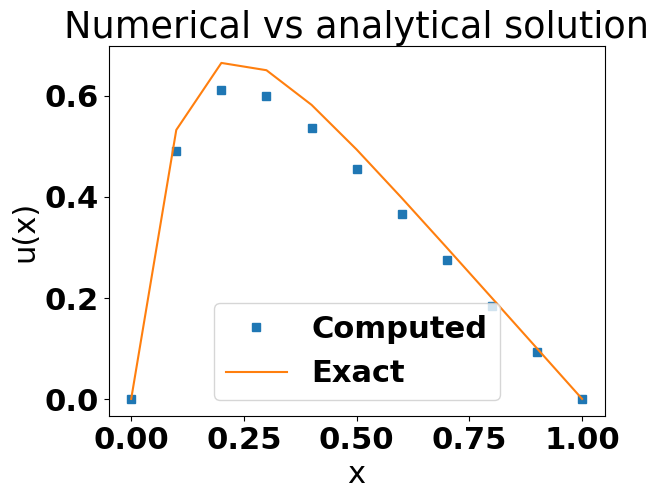
\includegraphics[width=0.4\textwidth]{images/gaussian_1.png}
    \caption{Numerical solutions plotted against the analytic solution for n=10. All figures are available in the Github repository}
    \label{fig:1}
\end{figure}

\begin{figure}[H]
    \centering
    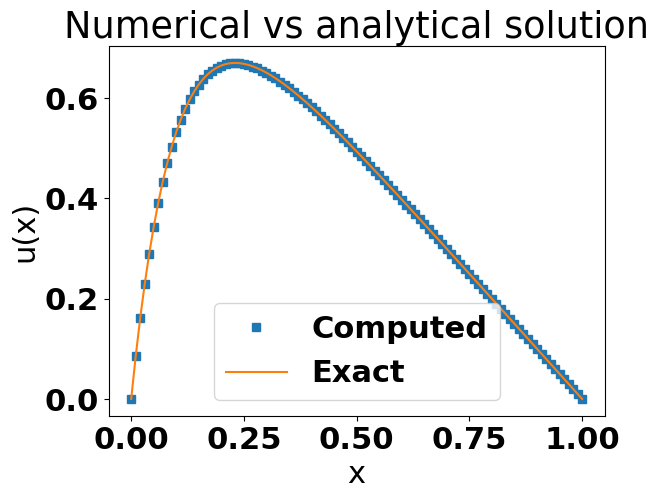
\includegraphics[width=0.4\textwidth]{images/gaussian_2.png}
    \caption{Numerical solutions plotted against the analytic solution for n=100. All figures are available in the Github repository}
    \label{fig:2}
\end{figure}

The error as a function of step size is also shown in figure \ref{fig:3}. We can see the error goes as a linear graph with slope 2, which shows in a logarithmic plot that the error scales as $h^2$.

This shows that a smaller step size is not always better, as we reach a minimum of error at step size $h=10^{-5}$. This is because for very small step sizes, the error in adding and subtracting nearly equal numbers increase, I.E. $u(x+h)+u(x-h)-2u(x)$ for our numerical derivative. We again divide this by $h^2$, further blowing up the error for small step sizes h, leading to loss of numerical precision. 

\begin{figure}[H]
    \centering
    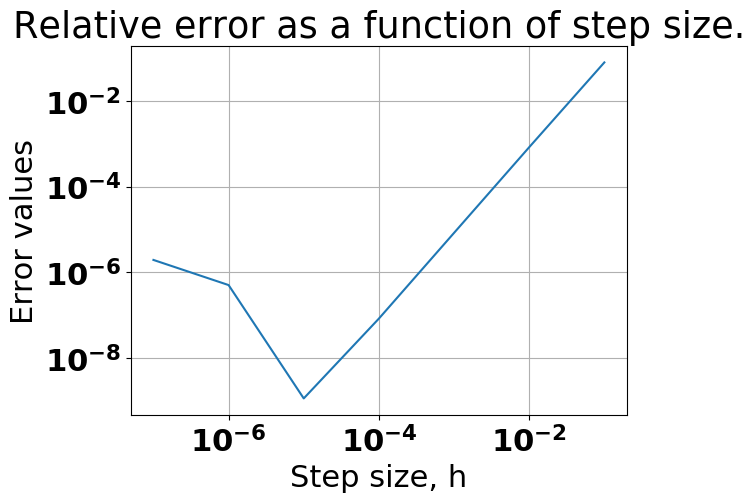
\includegraphics[width=0.4\textwidth]{images/RelativeError.png}
    \caption{Logarithmic plot of relative error plotted against step size.}
    \label{fig:3}
\end{figure}

\section{Conclusions}
\label{sec:conclusions}
The results in this letter shows that when faced with a set of linear equations, one has a lot to gain to tailor your algorithm to the special case you are dealing with. Saving CPU time by a factor of 2 is substantial, and comparing to the LU-decomposition, for which the CPU time differs by a factor of $~n^2$, tailoring the algorithm is absolutely essential.

We have also seen that for some cases, the problem is not even solvable by the standard LU-decomposition. For matrices with $n=10^5$ or above, we did not have enough memory to perform the algorithm. However, the tailored methods work just fine, since we do not have to construct a whole matrix. 

\pagebreak

\subsection{Further research}
In this letter we have focused on the Poisson equation, with a specific second order approximation. However, similar analysis can be done for several other types of equations, or different approximations. There would be a lot to gain by gaining as efficient methods as possible for each specific case, so that bigger and more complex systems can be simulated and analyzed. 

\begin{thebibliography}{}
\bibitem[(Hjorth-Jensen, 2018)]{MHJ} Hjorth-Jensen, Morten \, Sep 6 2018, "Computational Physics Lectures: Linear Algebra"
methods, http://compphysics.github.io/ComputationalPhysics/doc/pub/linalg/pdf/linalg-beamer.pdf

\end{thebibliography}

\section{Appendix}
All source code, data and figures can be found at the github repository: https://github.com/bruce-chappell/FYS4150/tree/master/project1

\end{document}
